\chapter{実験}
予備実験を含め,行なった実験は9種類ある.
予備実験として,DCADとレスキュー犬訓練データセットの2種類のクラス分類を行なった.
本実験では,
静止画像からのマルチラベル推定,
optical flow画像からのマルチラベル推定,
音声データからのマルチラベル推定2種,
Sound based Two-stream networkを用いた音声データと静止画像からのマルチクラス推定,
同じくSound based Two-stream networkを用いた音声データとoptical flow画像からのマルチクラス推定,
そしてSound based Three-stream networkを用いた音声データと静止画像とoptical flow画像からのマルチクラス推定の7種類を行なった.
\section{予備実験:クラス分類}
DCADとレスキュー犬訓練データセットについて,それぞれクラス分類を行なった.
DCADはクリップ毎にフレーム間の平均をとり,画像として扱ってVGG16のpretrained modelを用いてfinetuningを行なった.
レスキュー犬訓練データセットは動画をラベル毎に切り出して短いクリップ群を作り,そのクリップ毎に同様にフレーム間の平均を取った画像を作成しVGG16のpretrained modelを用いてfinetuningした.
\subsection{DCAD動画像平均画像クラス分類}
予備実験の結果を~(図\ref{vgg16_res}に示す.分類率は64.3\%であった.
全般的に,データの多いクラスは精度が高い傾向にあるが,データの少ないクラスは精度が低い傾向にある.
加えて,~\(Car\)クラスは道路の進行方向に対して垂直に待機している10クラスの中で特殊なクラスであり,車などの写ったフレームの影響で分類精度が上昇していると考えられる.~\(Feed\)クラス,~\(Pet\)クラス,~\(Play\_with\_ball\)クラスは,それぞれフレーム内を人間が占める割合が多いクラスと言え,そのため混同が起こりやすいと考えられる.

\begin{figure}[htbp]
 % \begin{tabular}{cc}
 %  \begin{minipage}{0.5\textwidth}
   \begin{center}

    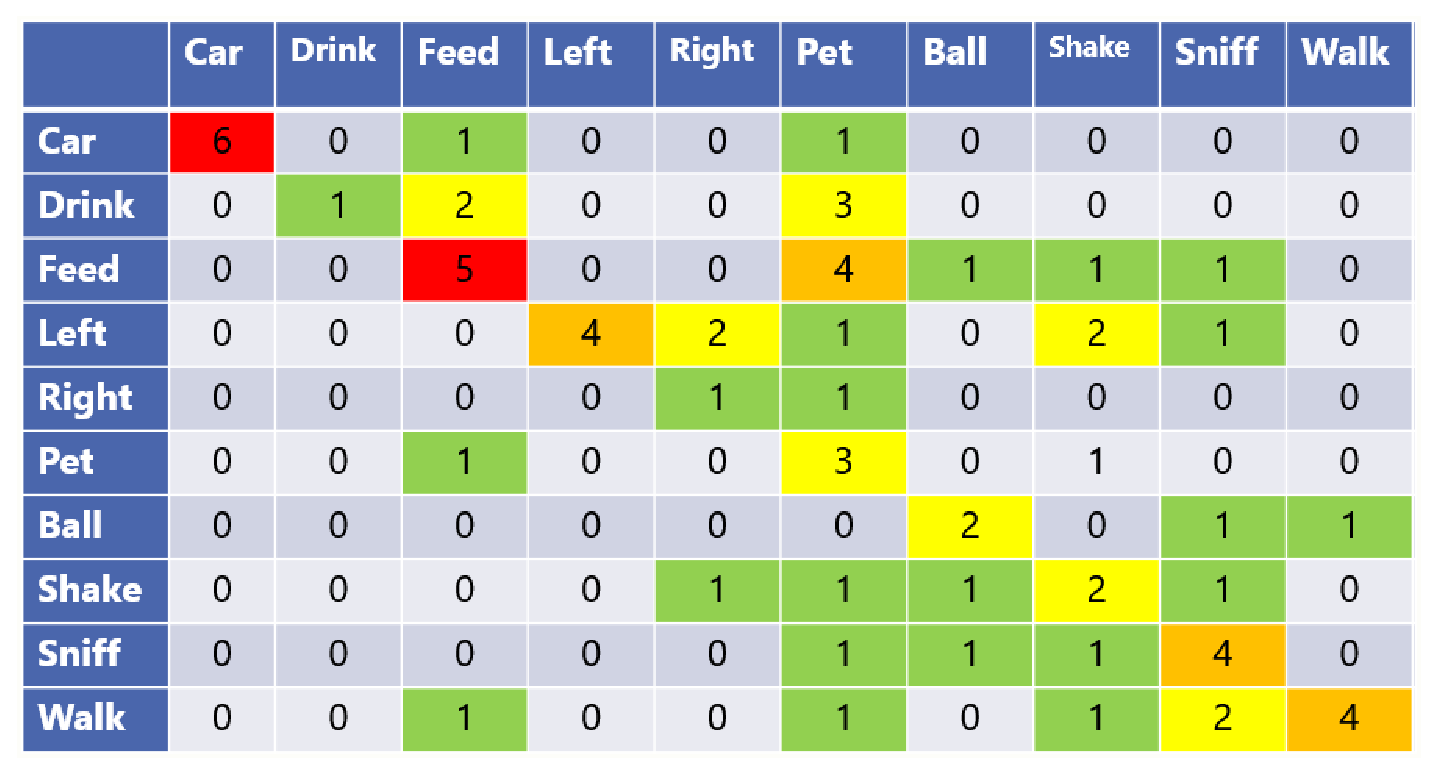
\includegraphics[scale=0.3]{./Figures/vgg16_res.eps}
    \caption{VGG16 pretrained modelによるfinetuningの結果}
    \label{vgg16_res}
   \end{center}
  % \end{minipage}
  % \begin{minipage}{0.5\textwidth}
\end{figure}

%% \subsection{レスキュー犬訓練データセット動画像平均画像クラス分類}
%% \begin{figure}[htbp]

%%    \begin{center}

%%     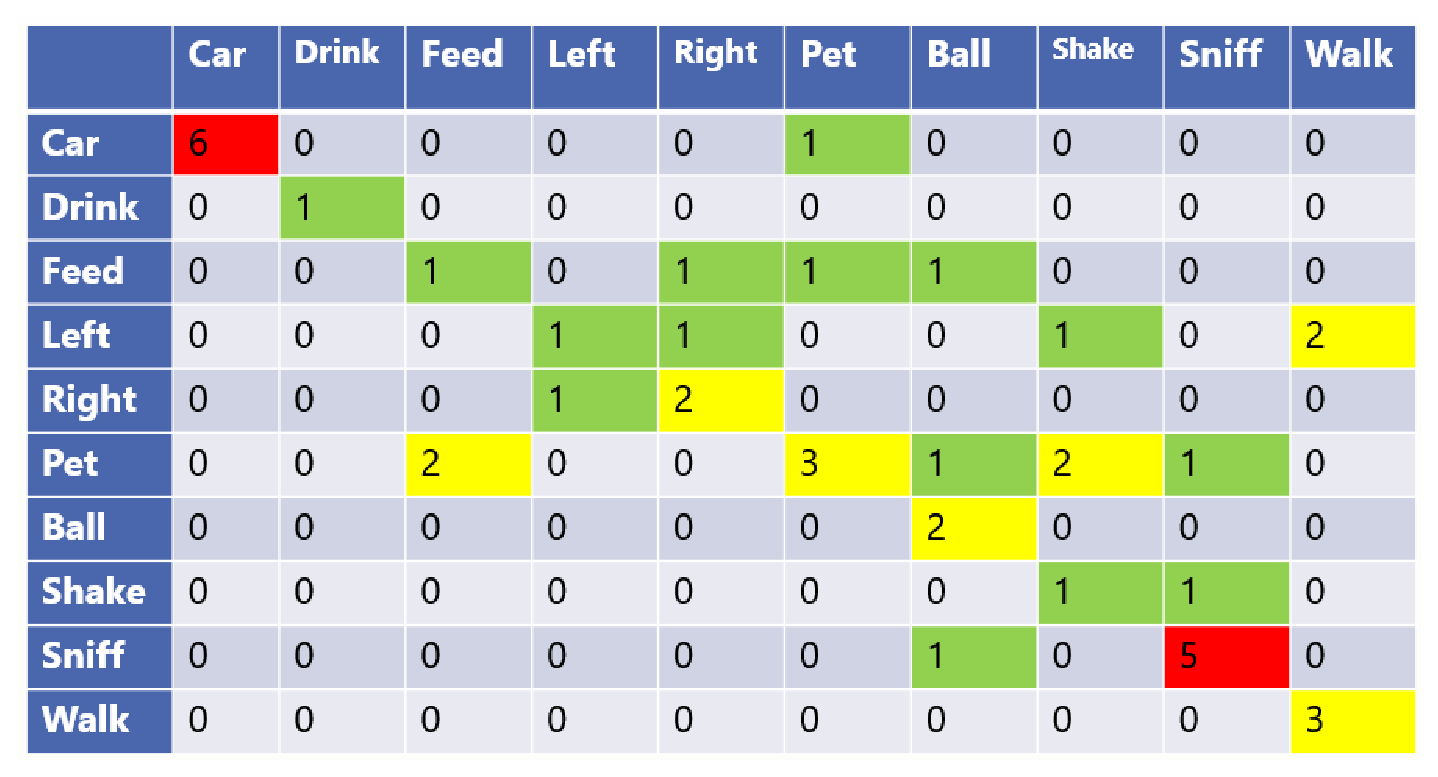
\includegraphics[scale=0.3]{./Figures/resnet_res.eps}
%%   \caption{ResNet pretrained modelによるfinetuningの結果}
%%   \label{resnet_res}
%%    \end{center}
%%  %  \end{minipage}
%%  % \end{tabular}
%% \end{figure}
%\section{オプティカルフロー動画平均画像クラス分類}
%動画像のフレーム間の平均を取った手法と同様に,クリップ毎にoptical flowの平均画像を作成しVGG16のpretrained modelを用いてfinetuningを行なった.
\subsection{レスキュー犬訓練データセット動画像平均画像クラス分類}

\subsubsection{2D Convolutional network}
音声データから得た(20, 94)次元の入力にチャネルを追加し,(20, 94, 1)の画像としてネットワークへ入力した.
1D Convolutional networkと比較し特徴量が増え,精度がわずかに上昇した.
推定精度を表~\ref{sound_2d_label}に示す.
全体としての精度は上昇したものの,クラス別に比較した際に1D Convolutional networkで学習したモデルに劣るクラスが半数近くを占める.
学習コストなどを含めるなど評価指標を変えた際には2D Convolutional networkが劣る可能性がある.
\begin{table}[tb]
 \centering
 \caption{音声データを用いた1d Convolutional networkの推定結果}\label{sound_2d_result}
 \scalebox{0.95}[1.00]{
  \begin{tabular}{|l||c|c|c|c|c|c|c|c|c|c|c|c|}
   \hline \hline
   クラス   & \rotatebox{90}{bark}& \rotatebox{90}{cling}&\rotatebox{90}{command}& \rotatebox{90}{eat}&\rotatebox{90}{handler}& \rotatebox{90}{run}&\rotatebox{90}{victim}& \rotatebox{90}{shake}& \rotatebox{90}{sniff}& \rotatebox{90}{stop}& \rotatebox{90}{walk} & \rotatebox{90}{全体}\\ \hline
Precision & 0.844& 0.094& 0.357& 0.013& 0.192& nan& 0.407& 0.794& 0.588& 0.917& 0.808&  0.639 \\ \hline
Recall    & 0.628& 0.064& 0.285& 0.002& 0.079& 0.0& 0.284& 0.33& 0.83& 0.797& 0.898&  0.721 \\ \hline
Jaccard   & 0.563& 0.04& 0.188& 0.001& 0.059& 0.0& 0.201& 0.304& 0.524& 0.744& 0.74&  0.512 \\ \hline


   % seven80_6fps_sound_bc-64_lr-0
%Precision & 0.86& 0.116& 0.243& 0.032& 0.194& 0.0& 0.375& 0.733& 0.565& 0.909& 0.766&  0.65 \\ \hline
   %Recall & 0.754& 0.333& 0.226& 0.006& 0.128& 0.0& 0.48& 0.524& 0.824& 0.742& 0.867&  0.642 \\ \hline
   %Jaccard & 0.672& 0.094& 0.133& 0.005& 0.083& 0.0& 0.267& 0.44& 0.504& 0.691& 0.686&  0.477 \\ \hline

  \end{tabular}
 }
\end{table}

\subsection{Two-stream network}
静止画像とoptical flow画像を学習していないVGG16ネットワークにそれぞれ入力し,得られた2つの出力を結合した結果からマルチクラス推定を行なった.
推定結果を表~\ref{stilloptic_result}に示す.
静止画像単体,optical flow画像単体からの推定と比較して精度がわずかに上昇している.
特にsniffクラスなどが劇的に精度が上昇している.動画から得られた静止画像の画像特徴に加えて,optical flowから得られる動き特徴をそれぞれ用いた学習ができていると考えられる.
ただし,shakeクラスなど,静止画像とoptical flow画像がお互いに悪影響を与え全く分類できなくなってしまったクラスも存在している.
\begin{table}[tb]
 \centering
 \caption{Two-stream networkの推定結果}\label{stilloptic_result}
 \scalebox{0.95}[1.00]{
  \begin{tabular}{|l||c|c|c|c|c|c|c|c|c|c|c|c|}
   \hline \hline
   クラス   & \rotatebox{90}{bark}& \rotatebox{90}{cling}&\rotatebox{90}{command}& \rotatebox{90}{eat}&\rotatebox{90}{handler}& \rotatebox{90}{run}&\rotatebox{90}{victim}& \rotatebox{90}{shake}& \rotatebox{90}{sniff}& \rotatebox{90}{stop}& \rotatebox{90}{walk} & \rotatebox{90}{全体}\\ \hline
Precision & 0.522& 0.04& 0.315& 0.0& 0.395& nan& 0.478& nan& 0.472& 0.848& 0.771&  0.571 \\ \hline
Recall    & 0.122& 0.033& 0.047& 0.0& 0.204& 0.0& 0.36& 0.0& 0.813& 0.807& 0.833&  0.646 \\ \hline
Jaccard   & 0.11& 0.018& 0.043& 0.0& 0.155& 0.0& 0.259& 0.0& 0.426& 0.705& 0.668&  0.435 \\ \hline

   % seven80_6fps_stilloptic_bc-128_lr-0_sr-5_sp-20

  \end{tabular}
 }
\end{table}
\subsection{Sound based Two-stream network}
音声データに静止画像,optical flow画像を個別に組み合わせ,マルチクラス推定を行なった.
音声の特徴を取り出すネットワークには2D Convolutional networkを用いた.
\subsubsection{音声データと静止画像からのマルチクラス推定}
音声と静止画像を組み合わせたマルチクラス推定の結果を表~\ref{stillsound_result}に示す.
\begin{table}[tb]
 \centering
 \caption{音声と静止画像からのマルチクラス推定結果}\label{stillsound_result}
 \scalebox{0.95}[1.00]{
  \begin{tabular}{|l||c|c|c|c|c|c|c|c|c|c|c|c|}
   \hline \hline
   クラス   & \rotatebox{90}{bark}& \rotatebox{90}{cling}&\rotatebox{90}{command}& \rotatebox{90}{eat}&\rotatebox{90}{handler}& \rotatebox{90}{run}&\rotatebox{90}{victim}& \rotatebox{90}{shake}& \rotatebox{90}{sniff}& \rotatebox{90}{stop}& \rotatebox{90}{walk} & \rotatebox{90}{全体}\\ \hline
  Precision & 0.909& 0.05& 0.312& 0.051& 0.249& 0.042& 0.42& 0.56& 0.592& 0.885& 0.787&  0.661 \\ \hline
Recall    & 0.709& 0.077& 0.341& 0.028& 0.177& 0.002& 0.537& 0.589& 0.758& 0.802& 0.855&  0.673 \\ \hline
Jaccard   & 0.662& 0.031& 0.195& 0.018& 0.115& 0.002& 0.308& 0.402& 0.498& 0.726& 0.694&  0.5 \\ \hline

   
   %seven80_6fps_stillsound_bc-32_lr-05
  \end{tabular}
 }
\end{table}
\subsubsection{音声データとoptidcal flow画像からのマルチクラス推定}
音声とoptical flow画像を組み合わせたマルチクラス推定の結果を表~\ref{opticsound_result}に示す.
\begin{table}[tb]
 \centering
 \caption{音声とoptical flow画像からのマルチクラス推定結果}\label{opticsound_result}
 \scalebox{0.95}[1.00]{
  \begin{tabular}{|l||c|c|c|c|c|c|c|c|c|c|c|c|}
   \hline \hline
   クラス   & \rotatebox{90}{bark}& \rotatebox{90}{cling}&\rotatebox{90}{command}& \rotatebox{90}{eat}&\rotatebox{90}{handler}& \rotatebox{90}{run}&\rotatebox{90}{victim}& \rotatebox{90}{shake}& \rotatebox{90}{sniff}& \rotatebox{90}{stop}& \rotatebox{90}{walk} & \rotatebox{90}{全体}\\ \hline
Precision & 0.887& 0.071& 0.332& 0.052& 0.245& 0.143& 0.329& 0.692& 0.564& 0.881& 0.791&  0.681 \\ \hline
Recall    & 0.729& 0.177& 0.441& 0.019& 0.198& 0.01& 0.409& 0.424& 0.782& 0.845& 0.847&  0.641 \\ \hline
Jaccard   & 0.667& 0.054& 0.234& 0.014& 0.123& 0.01& 0.223& 0.356& 0.487& 0.759& 0.692&  0.493 \\ \hline

%seven80_6fps_opticsound_bc-64_lr-0
  \end{tabular}
 }
\end{table}
\subsection{Sound based Three-stream network}
表~\ref{stillopticsound_result}に示す.
\begin{table}[tb]
 \centering
 \caption{still optic sound}\label{stillopticsound_result}
 \scalebox{0.95}[1.00]{
  \begin{tabular}{|l||c|c|c|c|c|c|c|c|c|c|c|c|}
   \hline \hline
   クラス   & \rotatebox{90}{bark}& \rotatebox{90}{cling}&\rotatebox{90}{command}& \rotatebox{90}{eat}&\rotatebox{90}{handler}& \rotatebox{90}{run}&\rotatebox{90}{victim}& \rotatebox{90}{shake}& \rotatebox{90}{sniff}& \rotatebox{90}{stop}& \rotatebox{90}{walk} & \rotatebox{90}{全体}\\ \hline
Precision & 0.888& 0.165& 0.282& 0.188& 0.313& 0.212& 0.527& 0.708& 0.621& 0.891& 0.822&  0.702 \\ \hline
Recall    & 0.623& 0.423& 0.355& 0.092& 0.306& 0.029& 0.709& 0.492& 0.783& 0.861& 0.86&  0.663 \\ \hline
Jaccard   & 0.577& 0.135& 0.186& 0.066& 0.183& 0.026& 0.433& 0.409& 0.53& 0.779& 0.725&  0.518 \\ \hline


%seven80_6fps_stillopticsound_bc-128_lr-0
  \end{tabular}
 }
\end{table}
